\chapter{補題3の検証}
本章では、\ref{hypothesis}節で定義した補題3を検証する。

\section{補題3}
\thirdLemma
% 外部の強制執行力が存在しない場合でも、成員の振る舞いによって強制執行力を自己組織化させることが可能である。

\section{提案手法}
各成員が「評判システム」を1つずつ所持している状態を仮定する。
補題2の検証で外部の強制執行力として存在していた「評判システム」を
ビザンチン将軍問題の署名付きの解法を用いて「分散型評判システム」として設計することで強制執行力の自己組織化を試みる。
この「評判システム」を所持している成員達のふるまいを記述し、
検証2と同様の結果になることをマルチエージェントシミュレーションを用いて検証する。

\section{分散型評判システム}
「評判システム」は、各成員の初期の「評判スコア」と報告された各時刻の約束の記録から現時刻の各成員の「評判スコア」を決定するシステムである。
各成員が「評判システム」を所有している場合、初期の「評判スコア」と各時刻の約束の記録が互いに共有されていれば、
各成員の所有する「評判システム」の現時点の各成員の「評判スコア」は一致する。

\subsection{仮定}
\begin{description}
  \item[仮定1] 送信されたすべてのメッセージは正しく到達する
  \item[仮定2] メッセージの受信者は誰が送信したのかわかる
  \item[仮定3] メッセージが届かないことを検知できる
  \item[仮定4] 誠実な成員の署名は偽造できず、署名されたメッセージの内容が変更されても、それを検知することができる。
  \item[仮定5] 誰でも成員の署名の信憑性を検証することができる。
\end{description}

\subsection{成員の振る舞い}
  \begin{itemize}
    \item 事前の合意に基づいて、全ての成員の人数$n$を決定する。
    \item 事前の合意に基づいて、各成員の初期の「評判スコア」$b_i, ..., b_n$を定義する。
    \item 事前の合意に基づいて、全ての成員が$promisor$と$reporter$のそれぞれの役割で総当りする周期を定義する。(周期の長さは$ n * (n-1)$)
    \item 事前の合意に基づいて、「評判システム」を用意する。
    \item 事前の合意に基づいて、約束の内容を定義する。
    \item 各時刻$t$において、「時刻tにおける成員の振る舞い」を上から順に実行する。
  \end{itemize}

\subsubsection{時刻tにおける成員の振る舞い}
\label{behaiverAtTimeT}
\begin{enumerate}
  \item 事前に合意した周期から$promisor$と$reporter$を決定する。
  \item $reporter$は時刻$t-n(n-1)$に$promisor$と交わした約束の結果を決定する。$t \leq n(n-1)$の場合、「履行」とする。
  \item $V_i=\emptyset$として初期化する。($\emptyset$は空集合)
  \item $reporter$は約束の結果を全ての成員に署名して送る。
  \item 各$i$について、 
  \begin{enumerate}
    \item もし$member_i$が$v:0$という形式のメッセージを受け取り、まだ何の報告も受けていない場合は、
    \begin{enumerate}
      \item $member_i$は$ V_i$を${v}$にする。 
      \item $member_i$は他のすべての成員にメッセージ$v:0:i$を送ります。
    \end{enumerate}
    \item もし$member_i$が$v:0:j_1:...:j_k$という形式のメッセージを受け取り、$v$が集合$V_i$に入っていない場合は
    \begin{enumerate}
      \item $member_i$は$v$を$V_i$に追加する。
      \item もし$k<m$であれば、$member_i$は$j_1, ..., j_k$以外のすべての副官に$v:0:j_1:...:j_k:i$というメッセージを送る。
    \end{enumerate}
  \end{enumerate}
  \item 各$i$について、$member_i$がこれ以上メッセージを受け取らない場合、$member_i$は$choice(V_i)$を報告された結果とする。
  \item 各$i$について、$member_i$は報告された結果を自身の「評判システム」に記録する。
  \item $reporter$は$promisor$と新たな約束を交わす。
\end{enumerate}

\section{実験方法}
  「8種類のエージェント」(\ref{agentsForExperiments2}節)から重複問わずランダムに8体のエージェントを用意し
  「実験用の約束」(\ref{promiseForExperiments}節)を用いた試行を実施する。
  これをタイプAのエージェントが0〜7体を占める場合について、それぞれ8000回の試行が行われるまで繰り返し、
  「報告された履行率」と「真の履行率」を記録する。

  \subsection{実験用の約束}
  \label{promiseForExperiments}
  \begin{itembox}[l]{時刻$t$に交わす約束}
    $promisor$は約束を交わした時刻$t$から時刻$t+n(n-1)$まで「時刻$t$における成員の振る舞い」に従い\textbf{step 4}と\textbf{step 5}で$reporter$にメッセージを送る。
  \end{itembox}

  \subsection{8種類のエージェント}
  \label{agentsForExperiments2}
    A〜Hの8種類のエージェントを用意する。それぞれのエージェントは下記の性質に従う。
    (記述のない振る舞いについては「実験用の時刻tにおける成員の振る舞い」に従う。)
    \begin{itemize}
      \item[A] 完全に「成員の振る舞い」に従うエージェント
      \item[B] 必ず「履行」を報告するエージェント
      \item[C] 真の約束のと逆の結果を報告するエージェント
      \item[D] 必ず「反故」を報告するエージェント
      \item[E] \textbf{step 4}と\textbf{5}でタイプA,B,C,Dに結果を送らないエージェント
      \item[F] \textbf{step 4}と\textbf{5}でタイプA,B,C,Dに結果を送らず、必ず「履行」を報告するエージェント
      \item[G] \textbf{step 4}と\textbf{5}でタイプA,B,C,Dに結果を送らず、真の約束の結果と逆の結果を報告するエージェント
      \item[H] \textbf{step 4}と\textbf{5}でタイプA,B,C,Dに結果を送らず、必ず「反故」を報告するエージェント
    \end{itemize}

  \subsection{事前の合意内容}
    \begin{enumerate}
      \item プレイヤー数$n$を$8$とする。
      \item 初期の各成員の「評判スコア」${b_i, ..., b_n}$を全て$8$とし、各エージェントはそれに合意する。
      \item 各時刻$t$の$promisor$と$reporter$組み合わせの周期を$(1, 2), (2, 1), ..., (7, 8)$とする。(周期の長さは56)
      \item 「評判システム」の詳細は検証2のものと同様とする。
    \end{enumerate}

  \subsection{試行}
    \begin{enumerate}
      \item 現在の時刻$t$を$0$とする。
      \item 各エージェントは「事前の合意内容」に合意する。
      \item 時刻$t$を1進める。
      \item 各エージェントはその特性に則って振る舞う。
      \item 各エージェントの「評判システム」について、時刻$t$の入力によって誰の通貨保有量も0未満にならない場合、「報告された結果」を記録する。
      \item 各エージェントの「評判システム」について、時刻$t$の入力によって誰の通貨保有量も0未満にならない場合、「真の結果」を記録する。
      \item 時刻$t$が$1120$未満なら、\textbf{step 4}に戻る。
      \item 各エージェントの「評判システム」において、過去$56$回分の\textbf{step5}と\textbf{6}で記録された結果を集計し、それぞれ「報告された履行率」と「真の履行率」して記録する。
    \end{enumerate}

\section{評価}
サンプリングした結果を元に、全ての誠実なエージェント(タイプA)の「評判システム」において、
「報告されて履行率」と「真の履行率」がそれぞれ100\%になっている施行を「約束が必ず履行される状態に至った施行」とした。
この「約束が必ず履行される状態に至った施行」の割合と誠実なエージェントの人数をプロットしたものが図\ref{compex-system-002}である。
この図から補題2と同様に誠実なエージェントの人数が増えるにつれて約束が必ず履行される状態に至った割合が高くなり、
5人以上の場合はサンプリングした全てのケースで約束が必ず履行される状態に至っていることがわかる。

\begin{figure}[h]
  \begin{tabular}{cc}
    \begin{minipage}[t]{1\hsize}
      \centering
      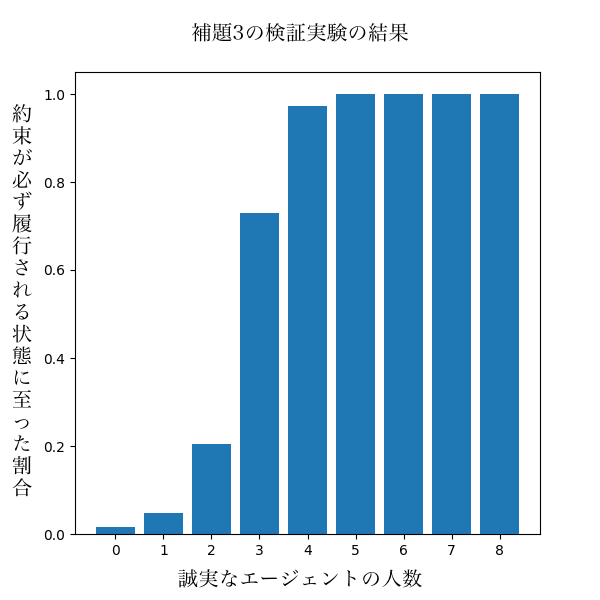
\includegraphics[keepaspectratio, width=1\linewidth]{./07_complex-system/figure01.png}
      \caption{誠実なエージェントの数と自己組織化に履行した割合}
      \label{compex-system-002}
    \end{minipage}
  \end{tabular}
\end{figure}

\section{補題3の結論}
実験と評価の結果から補題2の強制執行力は成員の振る舞いによって自己組織化することができ、
外部の強制執行力が存在しない場合でも、成員達が必ず約束を履行する状態に至れることがわかる。
また、それを用いてビザンチン将軍問題の署名付きの解法(\textbf{step 4}と\textbf{5})を守らない成員の「評判スコア」を下げることが可能である。
